\section[Theorie]{Theorie \textnormal{\cite{pumpen}}}
\label{sec:theorie}

Spätestens seit Einführung des Atommodells nach Bohr ist allgemein bekannt, dass sich Elektronenhüllen von Atomen aus
scharf definierten Energieniveaus zusammensetzen, deren Besetzung durch das Ausschließungsprinzip nach Pauli beschrieben wird.
Äußere Schalen sind nur teilweise oder gar nicht gefüllt und unterliegen dadurch zusätzlich der temperaturbedingten Verteilung
nach Boltzmann. Für Zustände mit $E_1 < E_2$ folgt
\begin{equation}
	\frac{N_2}{N_1} = \frac{g_2}{\rb{0.5ex}{$g_1$}} e^{-\frac{E_2 - E_1}{k_B T}}
	\label{eqn:besetzung}
\end{equation}
als das erwartete Verhältnis der Besetzungszahlen mit $k_B$ als Boltzmannkonstante und $T$ als absolute Temperatur. Die Faktoren
$g_1$ und $g_2$ geben als statistische Gewichte die Multiplizität oder Entartung der jeweiligen Energien $E_1$ und $E_2$ an.

Im thermischen Gleichgewicht gilt bei $g_1 = g_2$ also typischerweise $N_1 > N_2$ für äußere Niveaus. Die Beschreibung von Rubidium
fällt in diesem Kontext besonders leicht, da nur ein Elektron in einer nicht vollständig gefüllten Schale liegt \cite{rubidium}.
Unter Energieaufwand und bei passender Niveaustruktur lässt sich diese Relation zu $N_1 < N_2$ umkehren. Beim optischen Pumpen
geschieht dies unter Einstrahlung von Lichtquanten, wobei die Photonenergie genau
\begin{equation}
	E_\gamma = h \nu = E_2 - E_1
	\label{eqn:photon}
\end{equation}
betragen muss, um ein Elektron in die nächsthöhere Schale zu heben. Hierbei geben $h$ die Planckkonstante und $\nu$ die Frequenz an.
Dieses Vorgehen erlaubt eine sehr präzise Messung niederenergetisches Strukturen innerhalb der Niveaus. Einige der so zugänglichen
Größen sollen für das stabile $^{85}\text{Rb}$ und den langlebigen Betastrahler $^{87}\text{Rb}$ \cite{rubidium} bestimmt werden. 
Dazu müssen gewisse Zusammenhänge zwischen Drehimpulsen und magnetischen Momenten im atomaren System bekannt sein.

\subsection{Atomare Drehimpulse}

Zur Untersuchung des Rubidiums müssen die relevanten Drehimpulsbeiträge verstanden werden. Abbildung \ref{fig:drehimpulse}
skizziert deren Verknüpfungen in geometrischer Form.

\begin{figure}[H]
	\centering
	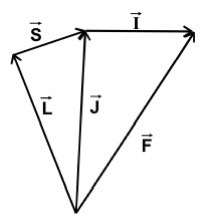
\includegraphics[width=0.25\linewidth]{content/grafik/drehimpulse.jpg}
	\caption{Vektordiagramm sämtlicher Drehimpulse eines Atoms. \cite{pumpen}}
	\label{fig:drehimpulse}
\end{figure}

Es lassen sich verschiedene Regionen unterscheiden, namentlich die Atomhülle und der Atomkern. Diese werden im folgenden 
genauer betrachtet.

\subsubsection{Hülle}

Aus den Eigenwerten der Drehimpulsoperatoren folgen mit $\bm{J} = \bm{S} + \bm{L}$ betragsweise
\begin{align*}
	\mu_J &= g_J \mu_B \sqrt{J(J + 1)} \\
	\mu_S &= g_S \mu_B \sqrt{S(S + S)} \\
	\mu_L &= \mu_B \sqrt{L(L + 1)}
\end{align*}
als zugehörige magnetische Momente mit dem Bohr Magneton
\begin{equation*}
	\mu_B = \pfrac{e \hbar}{2 m_e}
\end{equation*}
und den Quantenzahlen $J$ für den Gesamtdrehimpuls, $S$ für den Spin und $L$ für den Bahndrehimpuls. Mit $\mu_J$ wird der
Landé Faktor bezeichnet, der die Kombination aus $\mu_S$ und $\mu_L$ berücksichtigt. Im weiteren Verlauf werden
genauere Korrekturen aus der Quantenelektrodynamik vernachlässigt und der gyromagnetische Faktor des Elektrons $g_S = 2$
gesetzt. Zudem schränkt $|S - L| \leq J \leq |S + L|$ den erlaubten Wertebereich ein.

Solange äußere Magnetfelder klein genug sind um als Störung behandelt zu werden, wird das Gesamtmoment nach Russel und Saunders über
\begin{equation*}
	\bm{\mu}_J = \bm{\mu}_S + \bm{\mu}_L
\end{equation*}
als vereinfachte Kopplung ausgedrückt. Trigonometrische Überlegungen \mbox{führen schließlich}
\begin{equation}
	g_J = \frac{3 J (J + 1) + S(S + 1) - L(L + 1)}{2 J (J + 1)}
	\label{eqn:lande_J}
\end{equation}
für die geltende Beziehung ein. An dieser Stelle sei angemerkt, dass Alkalimetalle wie Rubidium ihren gesamten Hüllendrehimpuls
im einen äußeren Elektron \cite{rubidium} tragen. Daher kann in diesem Fall immer $S = \frac{1}{2}$ eingesetzt werden.

Beim Anlegen eines äußeren lokal homogenen Magnetfeldes $\bm{B}$ wird die zuvor arbiträre Basiswahl durch eine natürliche Symmetrie
ersetzt. Entlang der Feldrichtung präzidiert nun $\bm{\mu}_J$ und führt über Richtungsquantelung die Wechselwirkungsenergie
\begin{equation}
	E_Z = M_J g_J \mu_B B
	\tag{4a}
	\label{eqn:lin_zeeman_J}
\end{equation}
ein. Die Orientierungsquantenzahl $M_J$ gibt die Projektion von $\bm{J}$ auf die Feldachse an und läuft von $-J$ bis $J$ in
ganzzahligen Schritten. Auf diese Weise werden die Energieniveaus in $2J + 1$ Unterniveaus gespalten, der sogenannte Zeeman Effekt
tritt hier in linearer Form zum Vorschein.

\subsubsection{Kern}

Die beiden zu untersuchenden Isotope $^{85}\text{Rb}$ und $^{87}\text{Rb}$ besitzen mit den Quantenzahlen $I_{85} = \frac{5}{2}$
und $I_{87} = \frac{3}{2}$ \cite{rubidium} zusätzlich einen jeweils von Null verschiedenen Kernspin, dessen Einfluss wie in
Abbildung \ref{fig:drehimpulse} aufgezeigt per $\bm{F} = \bm{J} + \bm{I}$ im Drehimpuls des gesamten Atoms inkludiert werden muss.
Dabei liegt $F$ ganzzahlig zwischen $|J - F|$ und $|J + F|$ mit einer zu $J$ analogen Zeeman Aufspaltung. Statt
\eqref{eqn:lin_zeeman_J} gilt nun
\begin{equation}
	E_Z = M_F g_F \mu_B B
	\tag{4b}\stepcounter{equation}
	\label{eqn:lin_zeeman_F}
\end{equation}
mit $-F \leq M_F \leq F$ und dementsprechend $2F + 1$ Unterniveaus.

\begin{figure}[H]
	\centering
	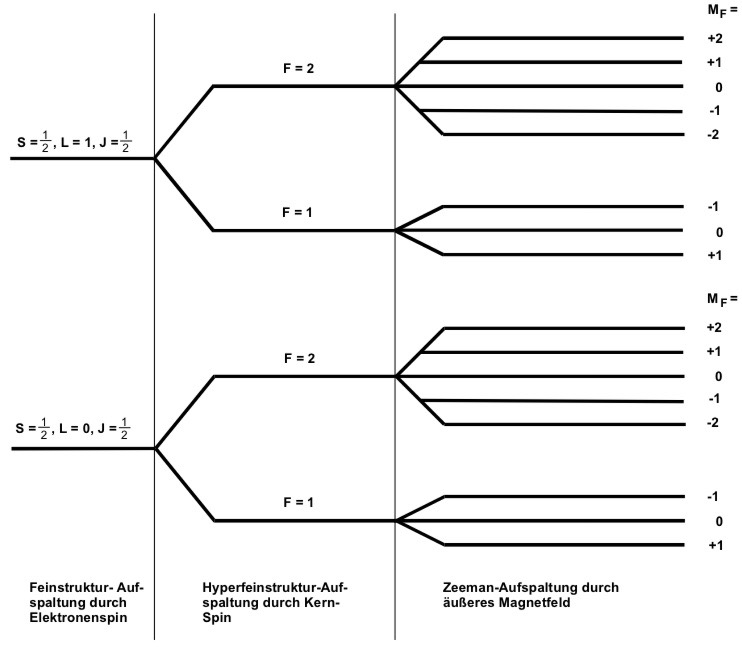
\includegraphics[width=0.7\linewidth]{content/grafik/hyperfein.jpg}
	\captionsetup{width=0.95\linewidth}
	\caption{Exemplarisches Termschema von $^{87}\text{Rb}$ unter Einwirkung eines Magnetfeldes. Energiedifferenzen sind
			 nicht maßstabsgetreu und liegen im Bereich von \qty{1.5}{\eV} für die Feinstruktur und \qty{30}{\micro\eV} für
			 die Hyperfeinstruktur. \cite{pumpen}}
	\label{fig:hyperfein}
\end{figure}

In Abbildung \ref{fig:hyperfein} wird beispielhaft eine resultierende Niveauaufspaltung dargestellt. Durch einen Ansatz der Form
\begin{equation*}
	\mu_F = g_F \mu_B \sqrt{F(F + 1)}
\end{equation*}
ergibt sich nach ähnlicher Rechnung zu \eqref{eqn:lande_J} schließlich
\begin{equation}
	g_F = g_J \,\frac{F (F + 1) + J(J + 1) - I(I + 1)}{2 F (F + 1)}
	\label{eqn:lande_F}
\end{equation}
für den Landé Faktor des atomaren Gesamtdrehimpulses. Im Grundzustand gelten $L = 0$ sowie folglich $J = S = \frac{1}{2}$ um
aus \eqref{eqn:lande_F} die Vorhersagen
\begin{align}
	g_F^{85} &= \pfrac{1}{3} \label{eqn:vorhesage_85}\tag{6a}\\ 
	g_F^{87} &= \pfrac{1}{2} \label{eqn:vorhesage_87}\tag{6b}\stepcounter{equation}
\end{align}
für die jeweiligen oberen Zweige der Hyperfeinstruktur $F_{85} = 3$ und $F_{87} = 2$ zu treffen.

\subsection{Optisches Pumpen}

Die prinzipielle Funktionsweise des optischen Pumpens wird nun zunächst anhand eines vereinfachten Alkaliatoms ohne Kernspin
erklärt und im Anschluss auf die spezifische Anwendung übertragen. In einem solchen System sind der Grundzustand $^2S_{1/2}$
sowie die durch $LS$ Kopplung hervorgerufenen angeregten Zustände $^2P_{1/2}$ und $^2P_{3/2}$ wie in Abbildung \ref{fig:duplett}
angeordnet, wobei hier zur Anschaulichkeit auf eine korrekte Skalierung verzichtet wird.

\begin{figure}[H]
	\centering
	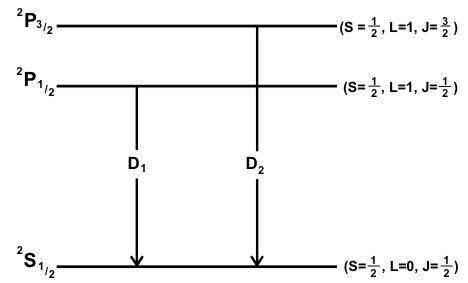
\includegraphics[width=0.5\linewidth]{content/grafik/duplett.jpg}
	\caption{Entstehung der Dublettstruktur in Alkalispektren. \cite{pumpen}}
	\label{fig:duplett}
\end{figure}

Die aufgezeigten Übergänge $D_1$ und $D_2$ erzeugen dann duplettartige Spektren wie sie für Alkalimetalle typisch sind.
Wird dazu ein Magnetfeld angelegt, spalten sich die ersten Niveaus nach Zeeman auf. Das resultierende Termschema ist zusammen
mit möglichen Übergängen in Abbildung \ref{fig:zeeman} skizziert.

\begin{figure}[H]
	\centering
	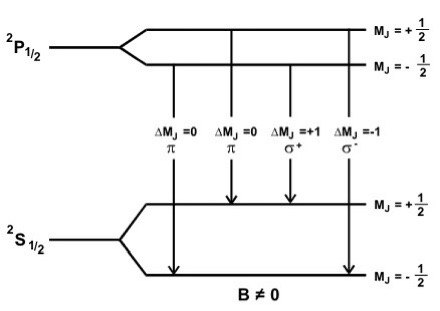
\includegraphics[width=0.55\linewidth]{content/grafik/zeeman.jpg}
	\caption{Zeeman Aufspaltung eines Alkaliatoms ohne Kernspin. \cite{pumpen}}
	\label{fig:zeeman}
\end{figure}

Da Photonen Spin $S = 1$ tragen, folgt aus Erhaltung des Drehimpulses, dass allgemein nur Übergänge mit $\Delta M_J = 0$ oder
$\Delta M_J = \pm 1$ möglich sind. Diese Auswahlregeln führen mit den eingeführten Bezeichnungen auf die Beschreibung des
mikroskopischen Polarisationszustandes durch Ausrichtung des Spins relativ zur Bewegung des Photons. Dabei entsprechen $\sigma^+$
und $\sigma^-$ je rechtshändig oder linkshändig zirkular polarisiertem Licht, also einer antiparallelen oder parallelen Helizität.
Im Fall von $\pi$ Emission liegt dagegen lineare Polarisation vor, durch den Dipolcharakter der Feldkonfiguration wird
davon jedoch keine Intensität entlang der Feldachse abgestrahlt.

Befindet sich nun eine mit diesen hypothetischen Alkaliatomen gefüllte und von einem homogenen Magnetfeld durchsetzte Dampfzelle
in einem Photonenfeld aus rechtshändig zirkular polarisierter $D_1$ Strahlung, erlauben die Auswahlkriterien die in Abbildung
\ref{fig:pumpen} markierten Übergänge.

\begin{figure}[H]
	\centering
	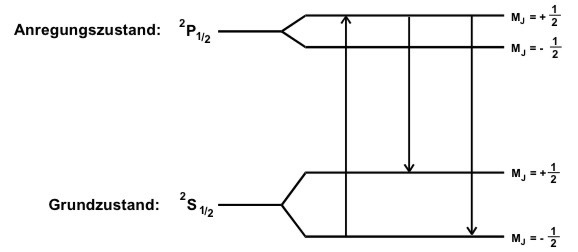
\includegraphics[width=0.65\linewidth]{content/grafik/pumpen.jpg}
	\caption{Mögliche Übergänge bei Einfall rechtzirkular polarisiertem Lichts. \cite{pumpen}}
	\label{fig:pumpen}
\end{figure}

Initial herrscht thermisches Gleichgewicht und die Besetzung ist wie in \eqref{eqn:besetzung} nach Boltzmann verteilt. Durch das
einfallende Licht werden die Elektronen aus dem niedrigesten $^2S_{-1/2}$ Zustand nach $^2P_{+1/2}$ angeregt.

Für Photonenemission an sich folgt $\Delta L = -1$ aus Drehimpulserhaltung, sodass die obere Population mit gleichen
Wahrscheinlichkeiten in $^2S_{-1/2}$ oder $^2S_{+1/2}$ abfallen kann. Da Elektronen aus dem $^2S_{+1/2}$
Zustand bei der gegebenen Lichtfrequenz allerdings nicht wieder angeregt werden und die Wahrscheinlichkeit für ein spontanes
Absinken in $^2S_{-1/2}$ verschwindend gering ist, wird das höhere der $^2S_{1/2}$ Zeeman Niveaus auf Kosten des niedrigeren
vollgepumpt. Der so entstehende makroskopische Zustand wird auch Besetzungsinversion genannt.

\begin{figure}[H]
	\centering
	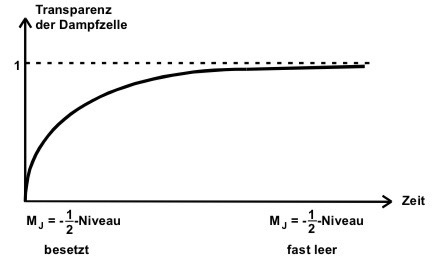
\includegraphics[width=0.6\linewidth]{content/grafik/transparenz.jpg}
	\caption{Zeitabhängige Transparenz einer Alkalidampfzelle. \cite{pumpen}}
	\label{fig:transparenz}
\end{figure}

Da die Anzahl der absorbierten
$D_1$ Photonen direkt von der Besetzung des so entleerten Grundniveaus abhängt, steigen Transparenz und Intensität wie
in Abbildung \ref{fig:transparenz} über
\begin{equation*}
	I = I_0 \left( 1 - e^{-t/\tau} \right)
\end{equation*}
mit der Zeit an, wobei $\tau$ eine unbekannte Zeitkonstante ist.

Real spielt auch der Kernspin der verschiedenen Isotope eine Rolle und führt zu deutlich mehr Zeeman Unterniveaus. Dazu kommt,
dass die Spektrallinien einer Gasentladungslampe der Dopplerverbreiterung unterliegen, sodass die feine Aufteilung sicher
abgedeckt ist. Die auftretenden Phänomene decken sich ansonsten aber hinreichend mit dem vereinfachten Fall.

\subsection{Zeeman Aufspaltung}

Der lineare Zeeman Effekt aus \eqref{eqn:lin_zeeman_J} und \eqref{eqn:lin_zeeman_F} muss für größere Magnetfeldstärken
in höherer Ordnung entwickelt werden. Mit der Hyperfeinstrukturaufspaltung $\Delta E_{HF}$ aus der Interaktion mit dem Kernspin
beschreibt
\begin{equation}
	\Delta E_Z = g_F \mu_B B + g_F^2 \mu_B^2 B^2 \frac{1 - 2M_F}{\Delta E_{HF}}
	\label{eqn:quad_zeeman}
\end{equation}
die Differenz benachbarter Unterniveaus in quadratischer Ordnung nach Breit und Rabi.

\begin{figure}[H]
	\centering
	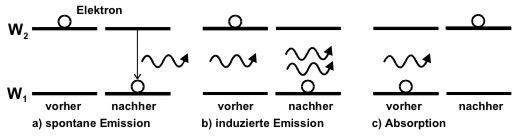
\includegraphics[width=0.75\linewidth]{content/grafik/uebergang.jpg}
	\caption{Übergangsmöglichkeiten eines Elektrons zwischen Energieniveaus. \cite{pumpen}}
	\label{fig:uebergang}
\end{figure}

Zum Verständnis der Präzisionsmessung sehr geringer Aufspaltungswerte müssen die beteiligten Übergangsmechanismen erläutert werden.
Abbildung \ref{fig:uebergang} stellt diese schematisch dar. Spontane Emission verläuft ohne Beteiligung äußerer Effekte. Selbst im
idealen Vakuum und ohne thermische Energie würden durch Quantenfluktuationen angeregte Zustände wieder auf energetisch günstigere
Niveaus abfallen. Dagegen erfolgt die stimulierte oder induzierte Emission durch resonante Wechselwirkung eines Photons mit dem
Dipolmoment übergehenden

\begin{figure}[H]
	\centering
	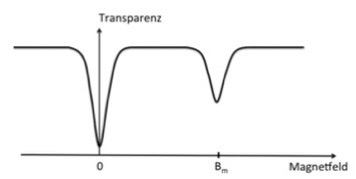
\includegraphics[width=0.6\linewidth]{content/grafik/minima.jpg}
	\caption{Transparenz einer Alkalidampfzelle unter Wirkung eines hochfrequenten Magnetfeldes in Anbhängigkeit
			 zur Feldstärke. \cite{pumpen}}
	\label{fig:minima}
\end{figure}

\subsection{Transiente Effekte}

\begin{equation}
	\omega = \pfrac{g_F\mu_B B}{\hbar}
	\label{eqn:larmor}
\end{equation}

\begin{figure}[H]
	\centering
	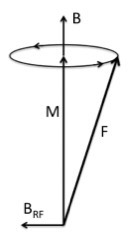
\includegraphics[width=0.2\linewidth]{content/grafik/praezession.jpg}
	\caption{Drehimpulspräzession um die Magnetfeldachse. \cite{pumpen}}
	\label{fig:praezession}
\end{figure}

